\documentclass[a4paper,12pt]{article}
\usepackage[utf8]{inputenc}
\usepackage{amssymb,amsmath,uniinput,graphicx,hyperref, multirow,siunitx}
\usepackage[section]{placeins}
\usepackage[ngerman]{babel}
\usepackage{feynmp}
\usepackage[left=3cm,right=3cm,top=3cm,bottom=3cm]{geometry}
\renewcommand{\familydefault}{\sfdefault}
\setlength{\belowcaptionskip}{6pt}
\hypersetup{pdfinfo = {
	Title={Versuchsprotokoll zu Produktion und Zerfall von W-Bosonen},
	Author={Knut Kiesel, Tobias Pook},
	Keywords={W-Bosonen}
}}

% for fenyman graphs
\setlength{\unitlength}{\textwidth}
\def\graphheight{0.15}
\def\graphwidth{.4}

% feynmf with pdflatex compability
\DeclareGraphicsRule{*}{mps}{*}{}

% missing transverse energy
\newcommand{\met}{\ensuremath{\not\mathrel{E}}_T}

% where to find graphics
\graphicspath{{../analyse/}}

\title{Laborpraktikum Teilchenphysik\\ DØ-Experiment: Produktion und Zerfall von W-Bosonen}
\author{Knut Kiesel\\Tobias Pook}
\date{\today}

\begin{document}
\maketitle
\vspace{3cm}
\tableofcontents
\thispagestyle{empty}
\newpage
\setcounter{page}{1}

\section{Ziel des Versuches}
\label{ziel}
Bei diesem Versuch werden aus Daten des DØ Detektors die Masse und die Zerfallsbreite des W-Bosons
sowie den Wirkungsquerschnitt zur Erzeugung und anschließendem Zerfall in zwei Leptonen bestimmt.

Um den Fund des W Bosons am UA2 Experiment zu bestätigen sowie es genauer zu Untersuchen können auch
beim DØ Experiment verschiedene Zerfallskanäle betrachtet werden. Einer von ihnen ist der Zerfall
in ein Elektron/Positron und ein Neutrino. Bei einer Erzeugung des W Bosons mit Valenzquarks der
Protonen/Antiprotonen ergibt sich der Feynmangraph in erster Ordnung in Abbildung
\ref{fig:feynman}.
\begin{figure}[h]
\centering
\begin{fmffile}{feymanE}
	\begin{fmfgraph*}(\graphwidth,\graphheight)
		\fmfleft{i2,i1}
		\fmfright{o2,o1}
		\fmf{fermion,label=$d$}{i1,v1}
		\fmf{fermion,label=$u$}{v1,i2}
		\fmf{photon,label=$W^-$}{v1,v2}
		\fmf{fermion,label=$ν$}{o1,v2}
		\fmf{fermion,label=$e$}{v2,o2}
	\end{fmfgraph*}
\end{fmffile}
\begin{fmffile}{feymanE+}
	\begin{fmfgraph*}(\graphwidth,\graphheight)
		\fmfleft{i2,i1}
		\fmfright{o2,o1}
		\fmf{fermion,label=$u$}{i1,v1}
		\fmf{fermion,label=$d$}{v1,i2}
		\fmf{photon,label=$W^+$}{v1,v2}
		\fmf{fermion,label=$e$}{o1,v2}
		\fmf{fermion,label=$ν$}{v2,o2}
	\end{fmfgraph*}
\end{fmffile}
\caption{Feynman Diagramm für die Erzeugung von W-Bosonen durch zwei Quarks der ersten Familie und
Vernichtung in zwei Leptonen.}
\label{fig:feynman}
\end{figure}

Den Wirkungsquerschnitt kann man mit
\begin{align}
\label{form:xstot}
	σ_W = \int_0^1dx_p\int_0^1dx_{\bar{p}} \sum_{i,j} f_i(x_p)f_j(x_{\bar{p}}) \hat{σ}_W
\end{align}
berechnen, wobei
\begin{align*}
	\hat{σ}_W = \frac{1}{N_C}\frac{12π}{m_W^2}\frac{Γ_{qq'}Γ_{eν}}{Γ^2_W}
	\frac{ x_px_{\bar{p}} s Γ_W^2}{\left( x_px_{\bar{p}}s - m_W^2\right)^2 + m_W^2Γ_W^2}
\end{align*}
und
\begin{align*}
	Γ_{ff'} = \frac{N_C}{12} \frac{α}{\sin^2θ_W}m_W
\end{align*}
ist. Dabei sind $f_i$ die Patron-Dichte-Funktionen, $N_C$ die Anzahl an Farben und $\sqrt{s}$ die
Schwerpunktsenergie.
Unter der Annahme, das W kann nur in drei Leptonfamilien und zwei Quarkfamilien zerfallen (das
top-Quark ist zu schwer), kann man über obrige Formel die gesamte Zerfallsbreite des W ausrechnen:
\begin{align}
\label{form:width}
	Γ_W = 3Γ_{eν} + 2Γ_{ud}  = \frac{ 3+2N_C}{12} \frac{α}{\sin^2θ_W}m_W
\end{align}
Damit ergibt sich für
\begin{align}
\label{form:xscms}
	\hat{σ}_W = \frac{πα²}{12\sin^4θ_W} \frac{ x_px_{\bar{p}} s }{\left( x_px_{\bar{p}}s -
	m_W^2\right)^2 + m_W^4\frac{(3+2N_C)^2}{12^2}\frac{α^2}{\sin^4θ_W}}.
\end{align}

Über die Masse des W Bosons kann man den elektroschwachen Mischungswinkel, oder auch Weinbergwinkel
$θ_W$ genannt, berechnen:
\begin{align}
	\label{form:wein}
	\cosθ_W = \frac{m_W}{m_Z}
\end{align}
In dem Versuch werden die Masse des Z Bosons $m_Z$ sowie die Feinstrukturkonstante $α$ als gegeben
vorausgesetzt.

\section{Vergleich von Simulation und Daten}

Im Detektor kann die W Masse nicht direkt gemessen werden, sondern nur manche Tochterteilchen. In
dem hier untersuchtem Prozess sind dies ein leichtes geladenes Lepton $e$
\footnote{Elektron wird ab nun als Synonym für Elektron und Positron benutzt} sowie
ein Neutrino $ν$
\footnote{Neutrino wird als Synonym für (Anti-)elektronneutrino benutzt}. Da die
longitudinale Anfangsbedinungen nicht bekannt sind, werden
nur transversale kinematische Größen betrachtet. Für die Auswertung werden Daten aus dem Kalorimeter
denen des Spurdetektors bevorzugt, da der Kalorimeter die kleinere Unsicherheit hat. So wird zum Beispiel
die transversale Energie eines Elektrons/Positrons
\begin{align*}
	E_{T} = E\sin\left( 2\arctan\left( e^{-\eta} \right) \right)
\end{align*}
aus der Energie im Kalorimeter $E$ und $\eta$ berechnet, wobei $\eta$ sowohl Informationen aus
Spurdetektor und Kalorimeter enthält.
Die Fehlende Transversale Energie wird komplett aus dem Kalorimeter bestimmt und berechnet sich
durch
\begin{align*}
	\met = \sqrt{ \not\mathrel{E}^{2}_{x} + \not\mathrel{E}^{2}_{y}}
\end{align*}
wobei $\not\mathrel{E}$ als
\begin{align*}
	\not\mathrel{E}_i = \left| - \sum E\vec{e_i} \right|
\end{align*}
definiert ist. Da das Neutrino im Detektor nicht nachgewiesen wird sondern ohne Interaktion den
Detektor verlässt, wird $\met$ als Neutrinoenergie
benutzt. Da nur die transversalen Komponenten von Elektron und Neutrino verwendet werden, kann auch
nur die invariante transversale Masse der Leptonen und damit des W Bosons berechnet werden.
\begin{align*}
	m_T = \sqrt{2E_T\met\left( 1-\cos(Δφ_{e,ν}) \right)}\hspace{0.3cm}\footnotemark
\end{align*}
\footnotetext{Da die beobachteten transversalen Elektronenergien größer als einige $\si{GeV}$ sind, wird
im Folgenden die Elektronmasse vernachlässigt.}

\subsection{Beschreibung der simulierten Daten}
Um Untergründe zu entfernen ist es hilfreich die gemessenen Daten mit simulierten Ereignissen zu
vergleichen. Da die W Masse im voraus noch nicht bekannt ist, werden Ereignisse für unterschiedliche
W Massen generiert.
Weil man den Untergrund durch $W\rightarrow τν_τ\rightarrow eν_τν_τν_e$ in Daten schlecht filtern kann,
sind auch $τ$ Ereignisse simuliert.

Die Qualität der Simulation ist aber eher durchwachsen, da gewisse Größen wie zum Beispiel der
Abstand des Vertices zum Ursprung, der Polarwinkel $φ$ oder die Elektronisolation sehr schlecht
beschrieben werden.

\begin{figure}[h]
	\centering
	\newcommand{\halftext}{0.49\textwidth}
	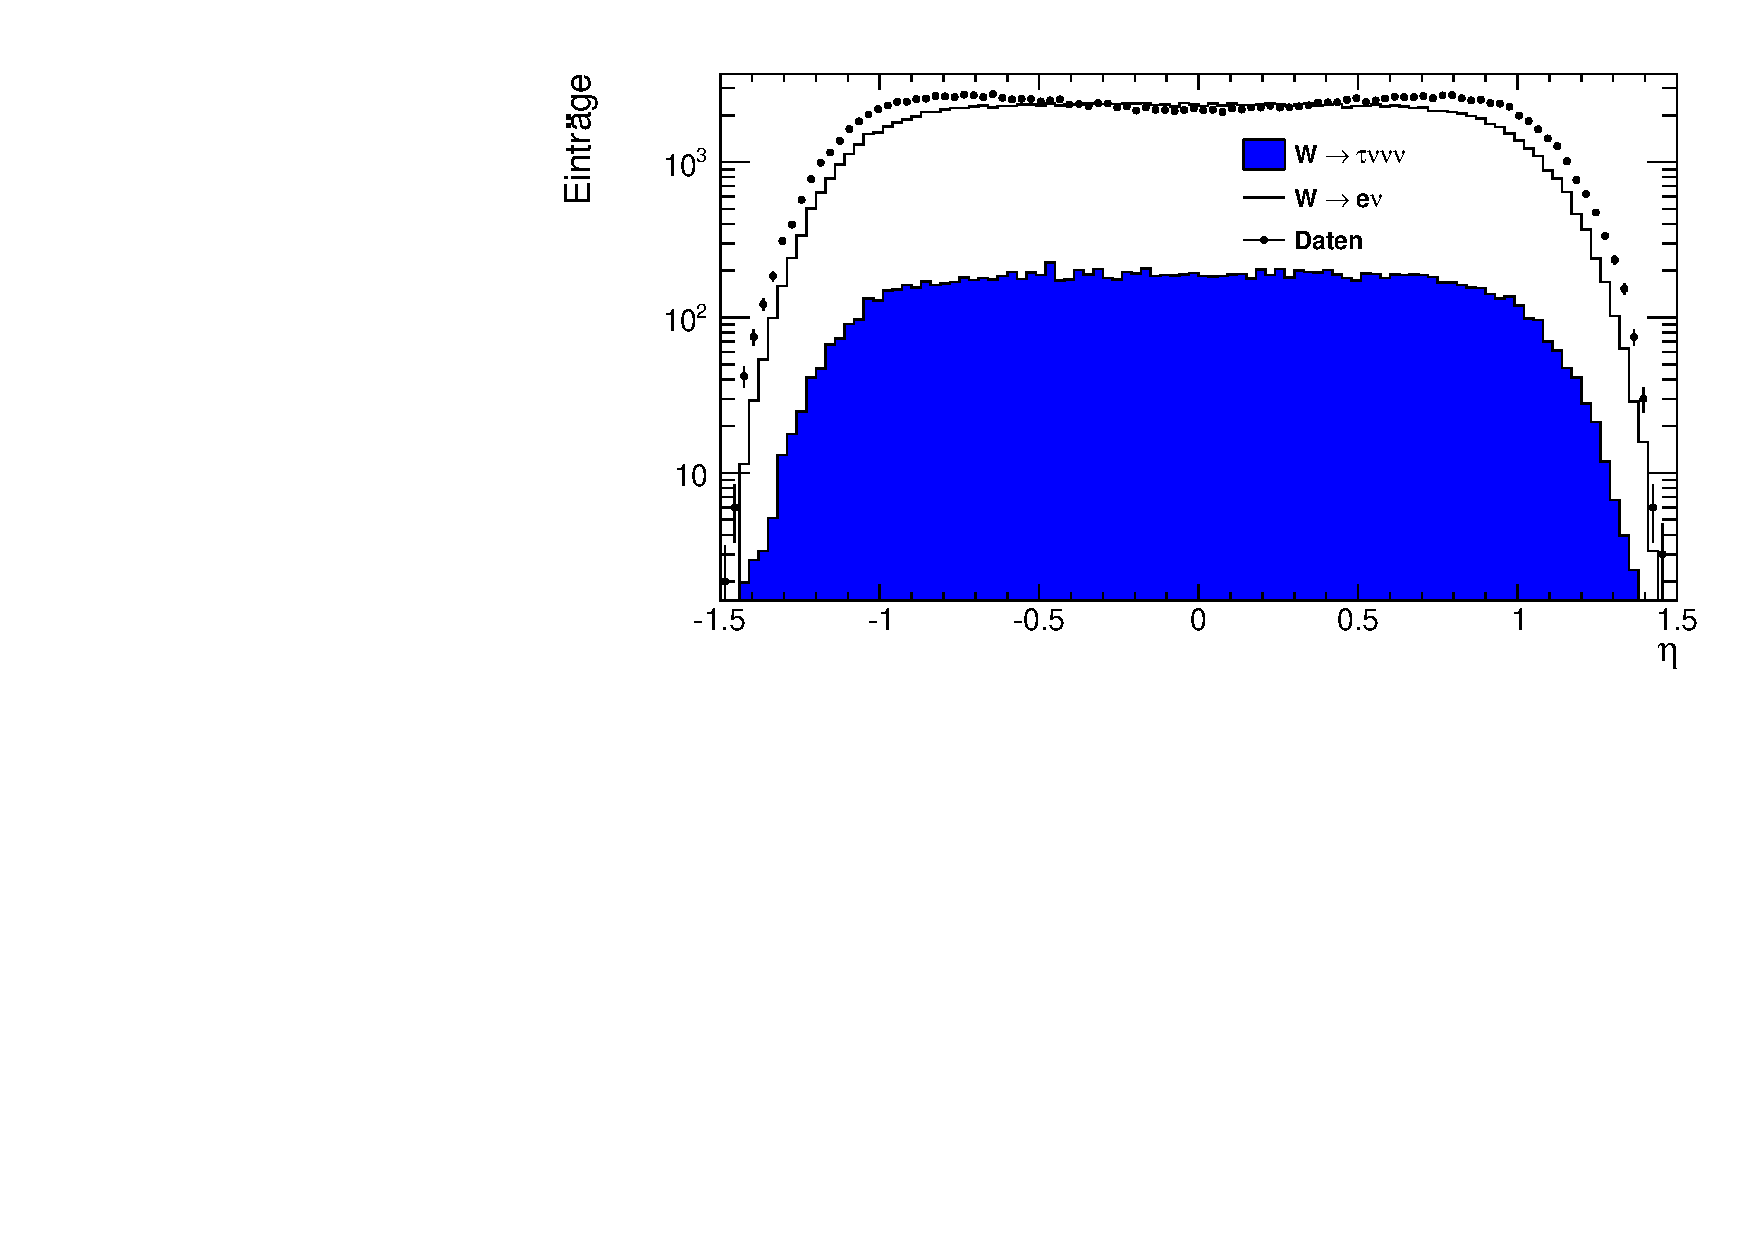
\includegraphics[width=\halftext]{eta.pdf}
	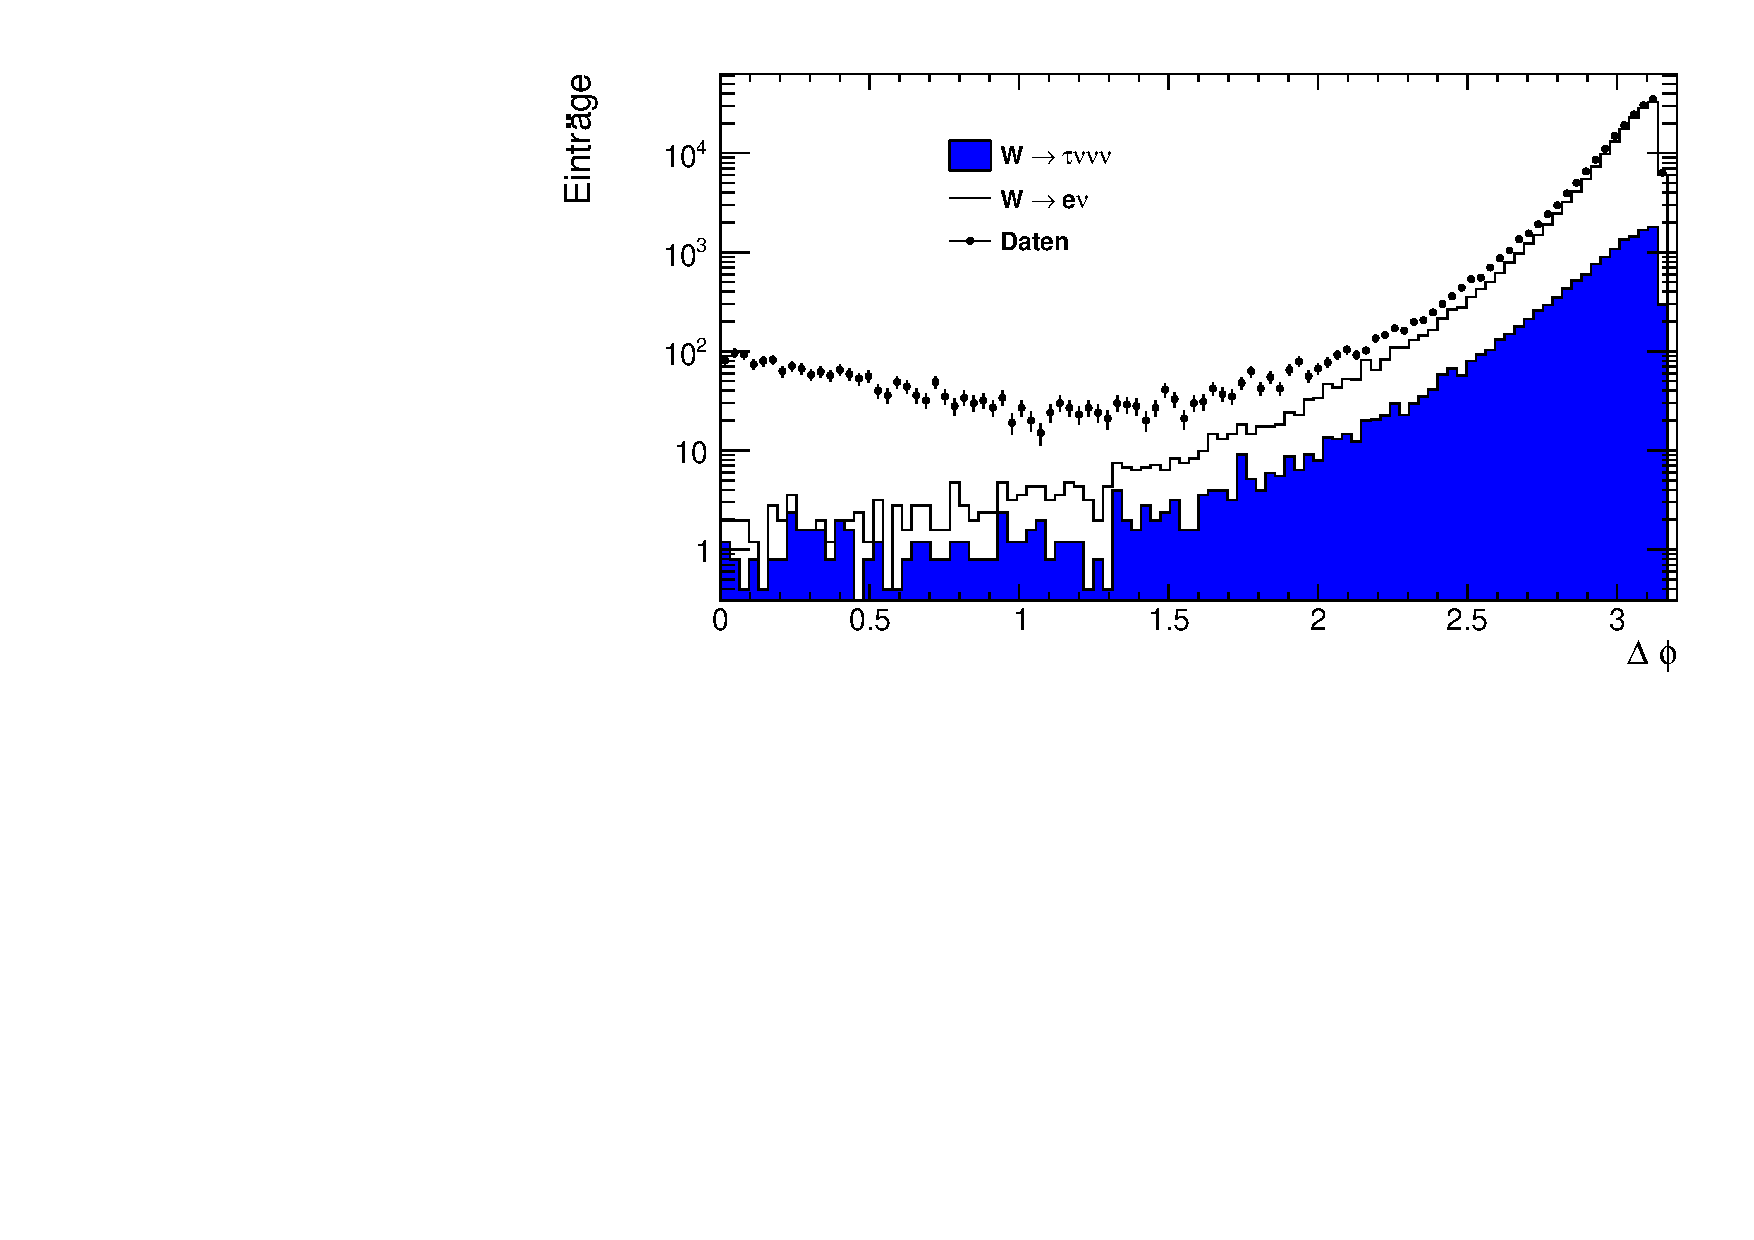
\includegraphics[width=\halftext]{delta_phi.pdf}\\
	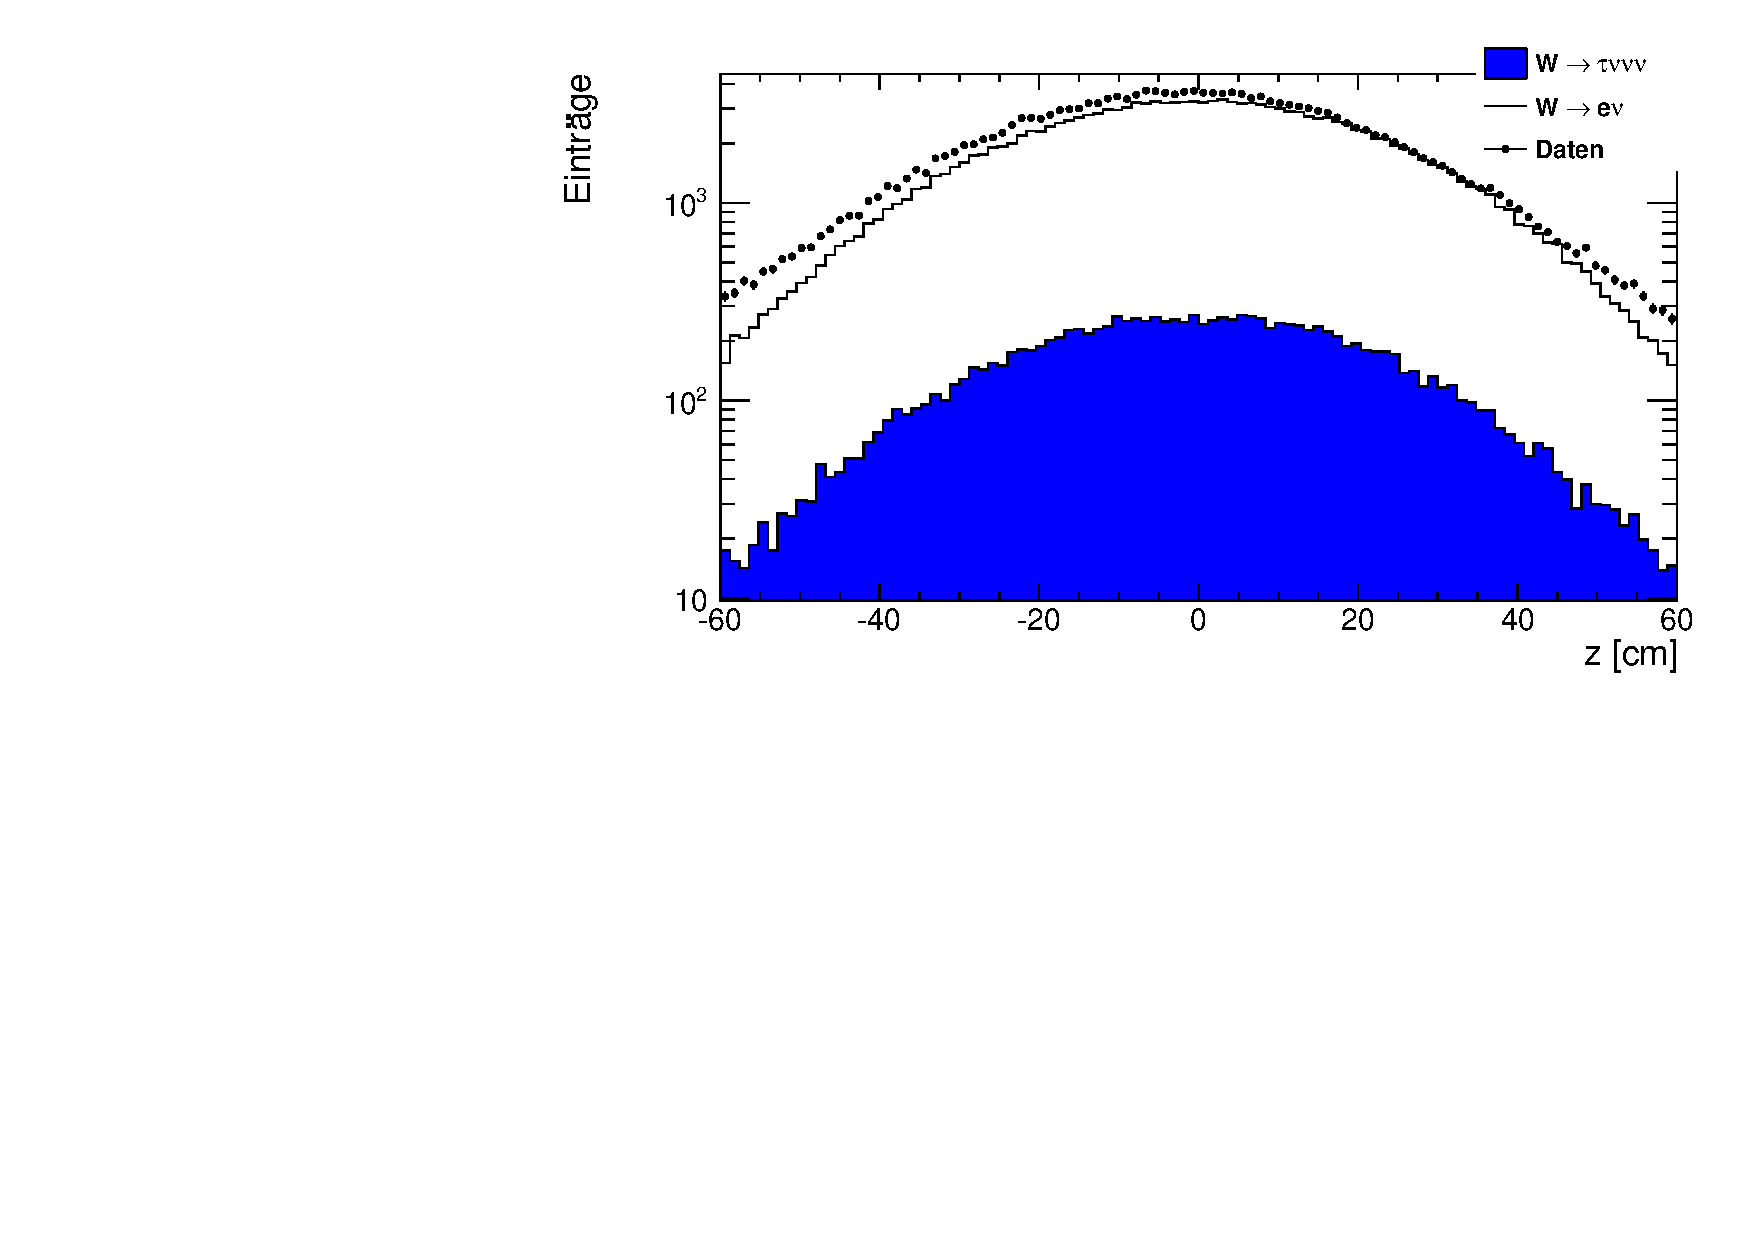
\includegraphics[width=\halftext]{vertex_z.pdf}
	\includegraphics[width=\halftext]{enengy_fraction.pdf}\\
	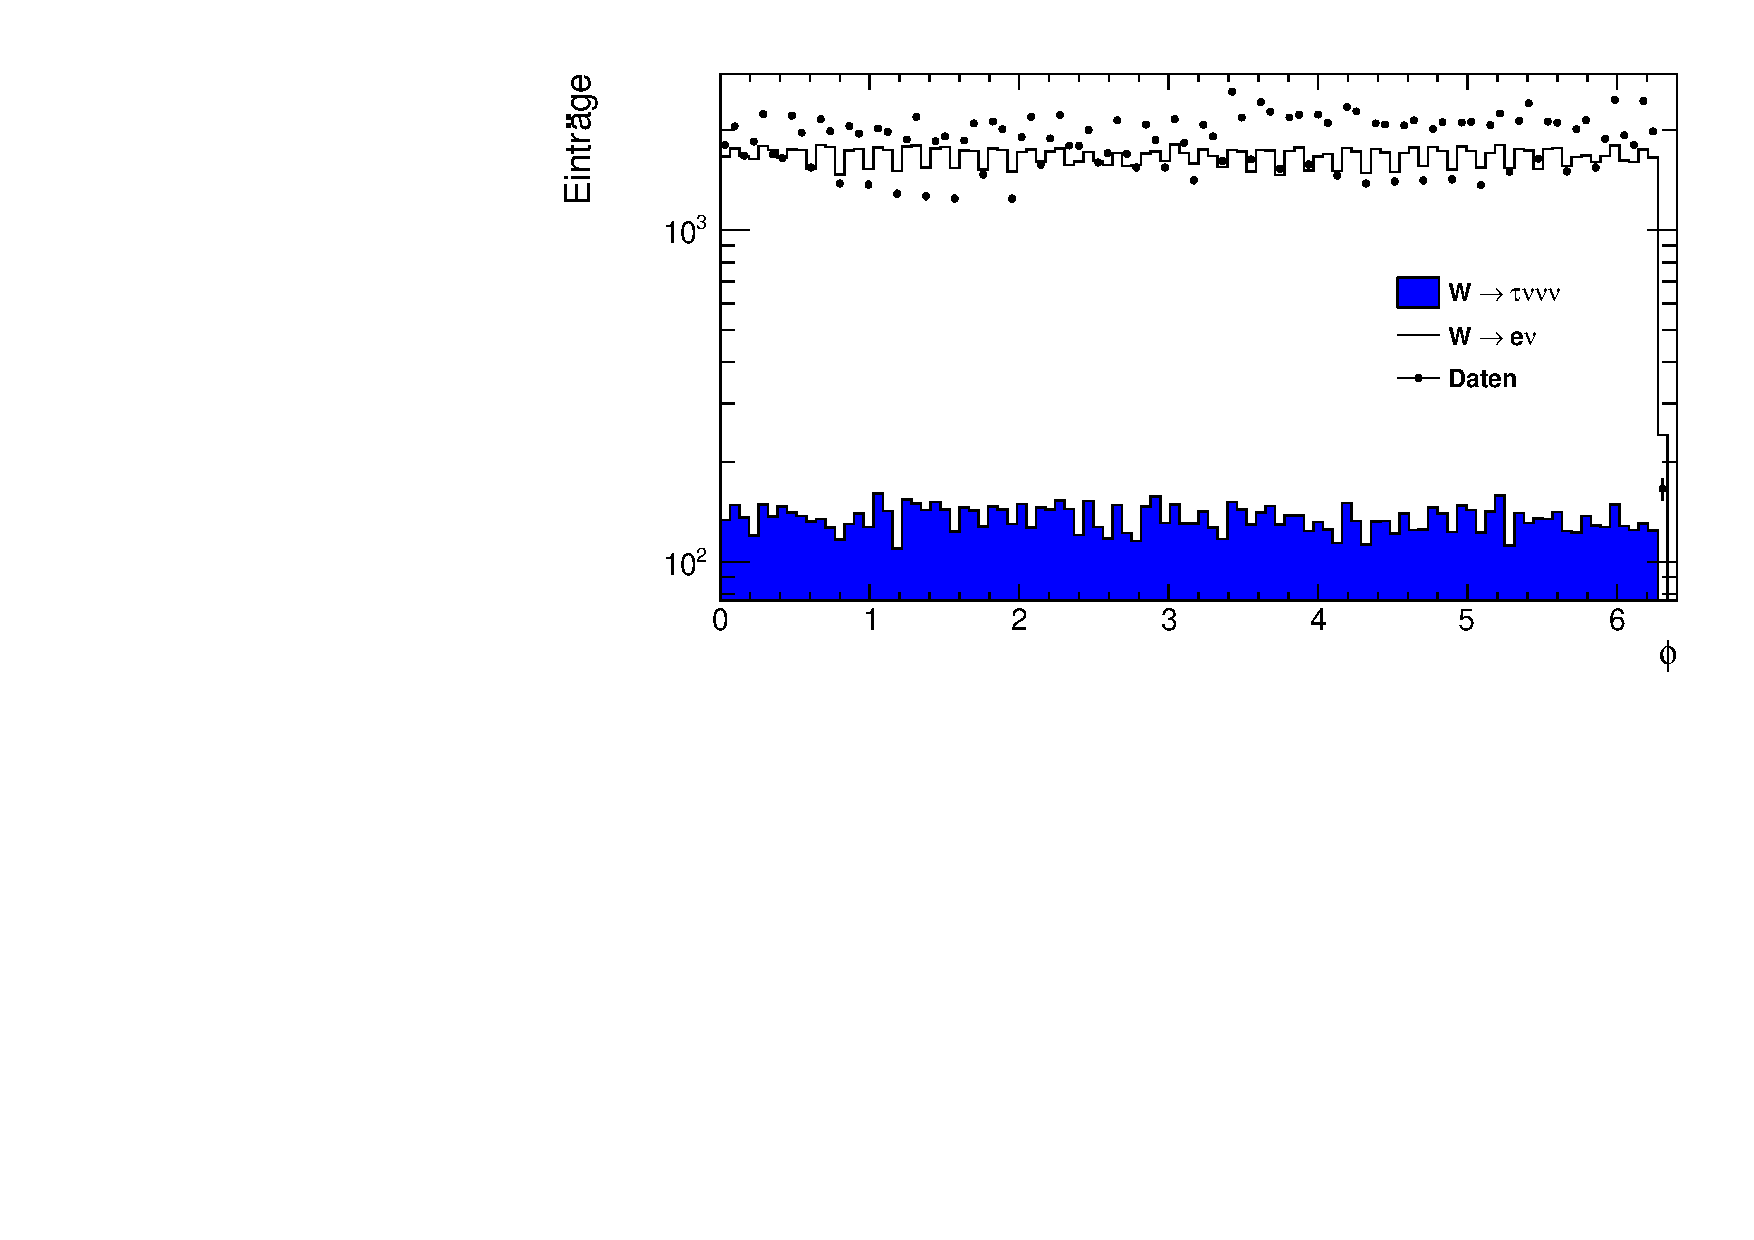
\includegraphics[width=\halftext]{phi.pdf}
	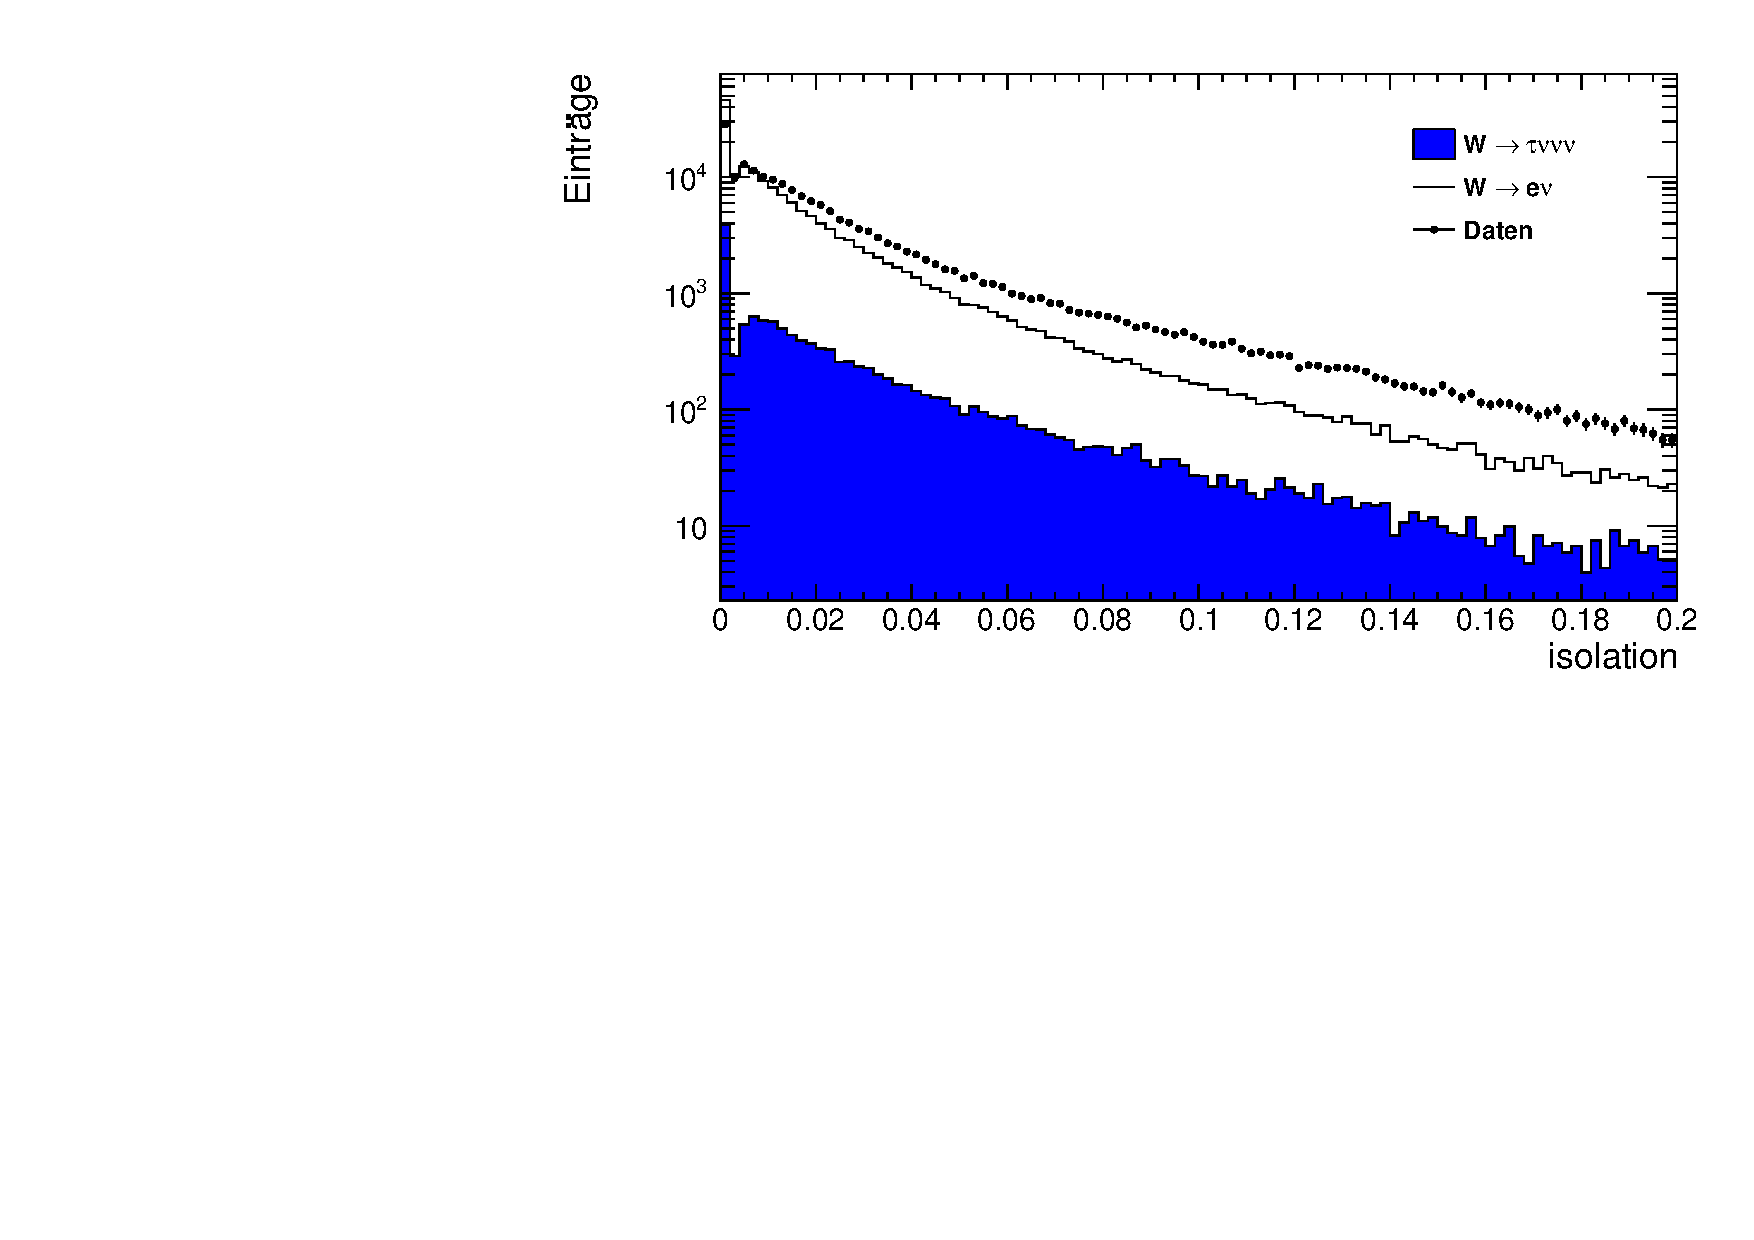
\includegraphics[width=\halftext]{isolation.pdf}\\
	\caption{Die Verteilung der Rapidität $η$, Winkel zwischen den Leptonen $Δ\phi$, der Abstand vom Ursprung in
	Strahlrichtung $z$, der Anteil der Energie im Kalorimeter, der Polarwinkel $\phi$ und die
	Elektronisolation für Daten und Simulation. }
	\label{fig:variables}
\end{figure}

Einige der Größen werden in Abbildung \ref{fig:variables} dargestellt. Man sieht die $τ$ Ereignisse
als blaues Histogram, die übrigen simulierten Daten als schwarzes Histogram und die Daten als
Punkte. 
\subsubsection*{Normierung der simulierten Daten}
Um einen Vergleich mit den gemessenen Daten zu ermöglichen, müssen die simulierten Ereignisse auf
die 
integrierte Luminosität der Daten von $\mathcal{L}_{int}=198 \pm \SI{20}{pb^{-1}}$ normiert werden.
Dazu werden die simulierten Ereignisse nach den Vorgaben aus der Versuchsanleitung\cite{versuchsanleitung}
in Abhängigkeit der Anzahl ursprünglich generierten Ereignissen$N_{gen}$ mit dem Faktor
\begin{align*}
	\textsl{w}= 0.9 \cdot \frac{\sigma \mathcal{L}_{int}}{N_{gen}}
\end{align*}
skaliert. Der Faktor $0.9$ beschreibt einen Korrekturterm, der eine im Vergleich zum realen Detektor
zu hoch angenommene Auflösung und Nachweiseffizienz bei der Generierung der Ereignisse berücksichtigt.


\subsection{Selektion der Daten}
Da nicht in allen aufgezeichneten Ereignissen der zu untersuchendem Prozess stattfindet, müssen die
Daten gefiltert werden, möglichst ohne viele richtige Ereignisse zu verlieren.
Um unerwünschte Ereignisse herauszufiltern, kann man Einschränkungen auf die Qualität der Daten (zum Beispiel
durch Isolationsschnitte) oder auf kinematische Größen festlegen.
Die die Qualität der gemessenen Daten durch die vorselektion gut ist, werden als Basisschnitte nur
die Schnitte der Anleitung gebraucht: Es werden nur
Elektronen betrachtet, deren Schauer wie eine elektromagnetische und nicht wie eine hadronische
Kaskade aussieht. Zu dem Schauer muss sich auch in kleinem Abstand eine Spur im Spurdetektor befinden.
Die Elektronen müssen isoliert sein, in $|\eta| < 1.1$ liegen. Es dürfen in dem Ereignis keine
hadronischen Jets mit einem Transversalimpuls von über $\SI{15}{GeV}$ vorkommen und der Primärvertex
darf entlang der Strahlachse nur $\SI{60}{cm}$ vom Mittelpunkt abweichen. Diese Auswahl wird immer
getroffen und nicht gesondert erwähnt wenn angewandt.

Die kinematischen Schnitte werden wie folgt bestimmt:
Die für eine bestimmte (beliebige) W-Masse simulierten und gemessenen Daten werden in normierte Histogrammen übereinandergelegt
und die Unterschiede durch geeignete Schnitte versucht zu verringert. Ziel ist vor allem eine gute
Übereinstimmung in $m_T$, da daraus zunächst die invariante Masse bestimmt wird. Die Abschätzung von Selektionsgrenzen
wird in Abbildung \ref{fig:abschaetzung} veranschaulicht. Links oben sieht man die transversale
invariante Masse ohne Einschränkungen. Die Verteilungen von Daten und Simulation unterscheiden sich
noch deutlich. Rechts oben sieht man die Verteilung der transversalen
fehlenden Energie. Da Daten und Simulation rechts der gezeichneten Linie gut übereinander stimmen,
wird in Zukunft gefordert, dass $\met > \SI{30}{GeV}$ sein muss. Im Bild links unten sieht man die
Verteilung der transversalen Elektronenergie mit der Einschränkung auf $\met$ und die Grenze, ab der Daten und Simulation hier
übereinstimmen. Zuletzt wird rechts unten wieder $m_T$ gezeigt. Die Übereinstimmung ist sehr viel
besser als am Anfang, die Simulation und Daten weichen kaum voneinander ab.

\begin{figure}[h]
	\centering
	\includegraphics[width=.49\textwidth]{mwt1tau.pdf}
	\includegraphics[width=.49\textwidth]{met1tau.pdf}\\
	\includegraphics[width=.49\textwidth]{el_etmet>30tau.pdf}
	\includegraphics[width=.49\textwidth]{mwtmet>30&&el_et>30tau.pdf}
	\caption{Abschätzung der Selektionsgrenzen mit Vergleich von Daten und Simulation. In Blau ist
	der $τ$ Untergrund eingezeichnet. Die Simulation entspricht hier einer W Masse von
	$\SI{80.3946}{GeV}$.}
	\label{fig:abschaetzung}
\end{figure}

In blau sieht man in jedem Bild Ereignisse, in denen das W ein $τ$ und ein $ν_τ$ erzeugt. Das $τ$
zerfällt nach sehr kurzer Zeit wieder in ein $e + ν_e + ν_τ$. Da man die Neutrinos nicht einzeln
Messen kann sondern nur die fehlende Energie, die durch alle Neutrinos zusammen verursacht wird,
kann man diese Ereignisse kaum Filtern, sondern muss den Untergrund über Simulationsvergleiche
abschätzen. Während am Anfang der Anteil der $τ$ Ereignisse noch 8.8\% beträgt, sind es nach beiden
Schnitten 1.1\%.

Da die wahre W-Masse unbekannt ist, kann man die Schnitte noch auf andere simulierte Datensätze
optimieren. Die Schnitte für die anderen W Massen ändert sich ungefähr um $\SI{5}{GeV}$, somit ist
dies unser Fehler.

Der Versuch auf die Elektronenisolation, den Abstand des Primärvertex oder ähnliche Variablen zu
schneiden wird aufgegeben, da es dort sehr schwer ist die Simulation und die Daten übereinander zu
bringen. Dies liegt unter anderem an der oben Beschriebenen schlechten Generation der Simulation.
Die gewählten Schnitte sorgen für ein gutes Übereinander stimmen von Daten und Simulation in den
kinematischen Größen, ohne dass die Effizient zu niedrig wird.

\newpage
\section{Bestimmung der Masse des W Bosons}
\subsection{Template Methode zur Bestimmung der W Masse}\label{cap:template}
Zuerst muss die Übereinstimmung von Simulation und Daten quantifiziert werden.

Da das Skalieren der simulierten Daten einen großen systematischen Fehler mit sich bringt und auch nach dem
Skalieren die gesamten Ereigniszahlen stark voneinander abweichen, ist es nötig, die Histogramme zu
normieren. Dies wiederum hat zur Folge, dass man den $χ²$ Test für gewichtete Histogramme anstatt
des normalen $χ²$ Test benutzen
muss\cite{cramer1999mathematical}.
Weiterhin müssen in einem Bin genug
Einträge sein (mehr als 9), damit man die poissonverteilten Einträge als eine Gaußverteilung nähern kann 
und man den Fehler als Quadratwurzel der Einträge benutzen kann. Außerdem verringert man
somit die relative Gewichtung von Bins mit zu wenig Einträgen.



Eine Schwierigkeit besteht weiterhin in dem Wählen der Anzahl der Bins sowie den verwendeten
Bereich der Variable, in der man die Übereinstimmung untersucht. Im Allgemeinen steigt das $χ²$ mit zunehmender Anzahl Bins. Die Anzahl der Bins wird auf
20 gesetzt, da dort der statistische Fehler klein ist, die Struktur der Verteilung aber nicht
verloren geht. Der Bereich wird möglichst groß gewählt, ohne dabei Bins mit weniger als 10 Einträge
mitzunehmen.

Trägt man nun für jede simulierte Masse das $χ²/\text{NDF}$ aus dem Vergleich zwischen der
Verteilung von $m_T$ von
Simulation und den Daten auf, erhält man wie in Abbildung \ref{fig:template} zu sehen eine Parabel.

\begin{figure}[htb]
	\centering
	\includegraphics[width=\textwidth]{template.pdf}
	\caption{Template Methode mit den Bedingung $\met > \SI{30}{GeV}$ und $E_{T} > \SI{30}{GeV}$. Die gesuchte W Masse befindet sich im Minimum der Parabel, da dort
		das $χ²/\text{NDF}$ minimal ist.}
	\label{fig:template}
\end{figure}
% minimum bei 1

Für die am Besten passende W Masse muss das $χ²/\text{NDF}$ möglichst klein sein. Man passt an den
Graphen in Abbildung \ref{fig:template} deshalb eine Parabel an und bestimmt deren Minimum. Die
Fehler sowie das $χ^2/\text{NDF}$ der Anpassung sind nicht von Bedeutung, da die Punkte keine
Fehler besitzen nur ein ROOT interner Standardfehler gesetzt wird und die Fehler auf die
Anpassungsvariablen zu berechnen.

Da das Minimum der Parabel nahe $1$ liegt, ergibt sich der statistische Fehler der W Masse aus der Abweichung vom Minimum beim Erhöhen des
$χ²/\text{NDF}$ um $1$.

Wenn man eine Parabel der Form $a + bx + cx²$ anpasst, erhält man somit $m_W = -\frac{b}{2c} ±
\frac{1}{\sqrt{c}}$.
Damit ergibt sich mit den Schnitten $\met > \SI{30}{GeV}$ und $E_{T} > \SI{30}{GeV}$
\begin{align*}
	m_W =  ( 80.25 ± 0.29  ) \si{GeV}.
	% aktuelle ausgaben von ./analyse ist nicht das gleiche
\end{align*}

Beim Variieren der Selektionsgrenzen, des Vergleichbereichs und der Anzahl Bins ändert sich der
eigentliche Wert der W Masse kaum, wohl aber der statistische Fehler. Er wird deshalb mit einer
Unsicherheit von $^{+0.8}_{-0.05}\si{GeV}$ abgeschätzt.Der Fehler auf diesen Wert wird im folgenden
vernachlässigt.
% ist der fehler auf den fehler in ordnung?
% wenn ja, später dazuschreiben, dass man ihn eh vernachlässigen kann, da der systemarische fehler
% größer ist

\subsection{Systematische Fehler bei der Bestimmung der W Masse}
\label{sysunc}
Im folgenden werden die berücksichtigten systematischen Fehler bei der W Massenbestimmung quantifiziert und zu einem systematischen Gesamtfehler
addiert.
\subsubsection*{Energieskala von $E_{T}$}
Die Bestimmung der Skala der Transversalenergie des Elektrons besitzt nach \cite{Abachi:1996ey} eine relative Unsicherheit von ca. $2\%$. Um den systematischen Einfluss
dieser Größe auf das Endergebnis zu bestimmen wurden alle $E_{T}$ Werte entsprechend dieser relativen Unsicherheit nach oben und unten variiert und die
W Masse erneut bestimmt. Die Abweichungen sind in Tabelle \ref{tab:syset} zusammengefasst. Damit lässt sich der mittlere systematische Fehler durch die
Wahl der transversalen Energieskala zu $\SI{0.98}{GeV}$ bestimmt.

\begin{table}[h]
	\centering
	\begin{tabular}{c| c c c}
		$\frac{\Delta E_{T}}{E_{T}}$ & $M_{W} [\si{GeV}]$ & $\Delta M_{W}[GeV]$ &$\frac{\Delta M_{W}}{M_{W}}$\\
		\hline
		$2\%$ & $81.16\pm 0.3$ & 0.91 & $1.1\%$\\
		$0\%$ & $80.25\pm 0.29$ & 0.0 & $0\%$ \\
		$-2\%$ & $79.21\pm 0.32$ & 1.04 &$1.3\%$
	\end{tabular}
	\caption{Änderung der W Masse bei Verschiebung der transversalen Elektronenenergieskala um die
	Energieunsicherheit von $2\%$.}
	\label{tab:syset}
\end{table}
\subsubsection*{Energieskala von $\met$}
Analog zum vorherigen Abschnitt wird nun auch die fehlende transversale $\met$ um $2\%$  variiert. Die Wahl dieser Abweichung wird dadurch begründet, dass
die gewählte Selektion hoch energetische Jets ausschließt und deshalb in der Berechnung von $\met$ die Unsicherheit
auf die Transversalenergie des Elektron eine dominante Rolle hat.
% falsch: wir haben hier nJets == 0 gefordert. met kommt hauptsächlich  durch die fehlenden
% leptonenenergien oder γ energien.

% Da steht das die Selektions'hoch energetische Jets außschliesst und deshalb die unsicherheit in met durch E_t (was bisher immer nur fürs Elektron genutzt wurde).
% Also genau das was du sagst. Wir haben ausserdem nicht NJet == 0 gefordert sondern lediglich keinen Jet > 15GeV Transversimpuls (siehe Anhang Versuchsanleitung) 


Die Ergebnisse der Variation sind in Tabelle \ref{tab:sysmet} zusammengefasst. Damit lässt sich der mittlere systematische Fehler durch die
Wahl der Energieskala der fehlenden transversalen Energieskala zu $\SI{0.98}{GeV}$ bestimmt.
\begin{table}[h]
	\centering
	\begin{tabular}{c| c c c}
		$\frac{\Delta \met}{\met}$ & $M_{W} [\si{GeV}]$ & $\Delta M_{W}$ &$\frac{\Delta M_{W}}{M_{W}}$\\
		\hline
		$2\%$ & $81.16\pm 0.3$ & 0.91 & $1.1\%$\\
		$0\%$ & $80.25\pm 0.29$ & 0.0 & $0\%$ \\
		$-2\%$ & $79.21\pm 0.32$ & 1.04 &$1.3\%$
	\end{tabular}
	\caption{Änderung der W Masse bei Verschiebung der fehlenden transversalen Energieskala um die
	Energieunsicherheit von $2\%$.}
	\label{tab:sysmet}
\end{table}

\subsubsection*{Variation der Selektionsgrenzen}
Um den Einfluss der gewählten Selektionsgrenzen zu bestimmen, werden diese um $\SI{5}{GeV}$
variiert. Es ergeben sich die Verschiebungen in Tabelle \ref{tab:variation}, mit denen der systematisch Fehler
auf die W Masse zu $\SI{0.35}{GeV}$ abgeschätzt wird, indem die halben Abweichungen quadratisch addiert werden.
\begin{table}[h]
	\centering
	\begin{tabular}{c| c c c}
		$E_{T} [\si{GeV}]$ gegen $\met [\si{GeV}]$ & 15 & 20 & 25 \\
		\hline
		25 &  & 80.27 & \\
		30 & 80.24 & 80.25 & 80.24 \\
		35 &  & 80.34 &
	\end{tabular}
	\caption{Änderung der W Masse bei Verschiebung der Selektionsgrenzen um $\SI{5}{GeV}$ um den
systematischen Fehler abzuschätzen.}
	\label{tab:variation}
\end{table}

\subsubsection*{Kombination der systematischen Fehlerquellen}
Das Berechnen des systematischen Gesamtfehler geschieht in zwei Schritten:
die Unsicherheiten auf $E_{T}$ und $\met$ sind, wie in Abbildung \ref{fig:etVSmet} zu erkennen ist, stark korreliert (Korrelationskoeffizient $0.85$)
% bei dem bild die schnitte anwenden, dann ist der korrelationskoeffizient noch näher bei 1
und werden deshalb zunächst linear addiert. Die Unsicherheit durch die Wahl der Selektionsgrenzen wird (auch wenn das sicherlich nicht ganz korrekt ist)
als unabhängig angesehen und zu dem gemeinsamen Fehler der Energieskalenbestimmung quadratisch addiert. Damit ergibt sich als abschließendes Ergebnis der
W Massenbestimmung:
\begin{align*}
	m_W = ( 80.32 ± 0.27 (stat.) ± 1.99(sys.)) \si{GeV}
\end{align*}
\begin{figure}[htb]
	\centering
	\includegraphics[width=\textwidth]{correlation_metVSel_et.pdf}
	\caption{Grafische Darstellung der Korrelation zwischen $E_{T}$ und $\met$ mit in rot eingezeichneten Selektionsgrenzen}
	\label{fig:etVSmet}
\end{figure}

\FloatBarrier
\subsection{Überprüfung der Ergebnisse durch Untersuchung einer Kontrollvariablen}
Um die Unsicherheiten der Analyse von $m_{T}$ besser abschätzen zu können und das Ergebnis zu überprüfen wird zusätzlich
die Übereinstimmung der $E_T$ Verteilungen verglichen und daraus mit der Template Methode die W Masse
berechnet. Eine einfache Mittelung der Werte ist nicht möglich, da $m_T$ und $E_T$ stark korreliert
sind, wie man in Abbildung \ref{fig:correlation} sehen kann.
\begin{figure}[htb]
	\centering
	\includegraphics[width=\textwidth]{correlation_mwtVSel_et.pdf}\\
	\includegraphics[width=\textwidth]{correlation_mwtVSel_etmwt_el_et>1_7.pdf}
	\caption{Korrelation zwischen $E_T$ und $m_T$ in der Simulation und in Daten, ohne Selektion
	(links) und mit einer Einschränkung auf das Verhältnis (rechts). Mehr zu dieser Grenze siehe
	unten.}
	\label{fig:correlation}
\end{figure}

% korrelationskoeffizienten mit e_t >30 cut wäre interessanter
Die Korrelationskoeffizieten sind 0.96 für die Simulation und 0.77 für die Daten. Man sieht hier
auch deutlich einen Unterschied  zwischen Simulation und Daten, der aber mit einem Schnitt auf $E_T$ bei
$\SI{30}{GeV}$ entfernt werden kann. Alternativ kann man auch auf das Verhältnis von $m_T$ zu $E_T$
schneiden, wie in Abbildung \ref{fig:verhaeltnis} zu sehen ist.

\begin{figure}[htb]
	\centering
	\includegraphics[width=1\textwidth]{mwt_el_et1tau.pdf}
	\caption{Vergleich der Verteilungen von $m_T/E_T$ zwischen Daten und Simulation mit
	Selektionsgrenze.}
	\label{fig:verhaeltnis}
\end{figure}

Wenn man diesen Schnitt anwendet, erhält man Abbildung \ref{fig:correlation} unten und man
erhöht den Korrelationskoeffizieten auf 0.97 für die Simulation und 0.94 für die Daten.

Bei Wahl der gleichen Selektionsgrenzen wie bei der Bestimmung von $m_{W}$ über $m_T$ zeigt sich, dass 
für $E_{T}$ eine wesentlich schwächere Übereinstimmung zwischen Daten und Simulation besteht, insbesondere
im Maximum des Peak (siehe Abbildung \ref{fig:etaftercut}).
\begin{figure}[htb]
	\centering
	\includegraphics[width=.7\textwidth]{E_t_aftercut.pdf}
	\includegraphics[width=.7\textwidth]{E_t_aftercut_peak.pdf}
	\caption{$E_{T}$ Verteilung nach der Selektion. Die gesamte Verteilung (oben) und ein Zoom auf das Maximum des Peak (unten) }
	\label{fig:etaftercut}
\end{figure}



%Um bessere Ergebnisse zu erzielen, wird der noch die oben beschriebene Selektion von $m_T/E_T < 1.7$ verwendet und es ergibt sich ein $χ²/\text{NDF}$
%von $1.004$. Durch das optimieren der Selektionsgrenzen auf $E_T$, $\met$ und $m_T/E_T$ erhält man
%eine W Masse von



\begin{figure}[htb]
	\centering
	\includegraphics[width=0.7\textwidth]{templateet.pdf}
	\caption{Ergebnis der Template Methode zur Bestimmung der W Masse für einen Vergleich der $E_{T}$ Verteilung}
	\label{fig:chiet}
\end{figure}
Das minimale $χ²/\text{NDF}$ der Template Methode ist in diesem Fall ca. $2.4$ (siehe Abbildung
\ref{fig:chiet}), dass heißt der durch die Methode bestimmte statistische Fehler wird
die tatsächlichen Fehler wohl unterschätzen. Da die Berechnung für $E_{T}$ jedoch nur zur Kontrolle der Ergebnisse in $m_{T}$ benutzt werden soll,
wird an dieser Stelle darauf verzichtet eine andere Selektion zu wählen um das $χ²/\text{NDF}$ näher an 1 zu bringen.

Die Bestimmung der systematischen Fehler erfolgt analog zu
Abschnitt \ref{sysunc}. Es ergeben sich systematische Abweichungen von $\SI{0.1}{GeV}$ für die Wahl der Selektionsgrenzen (siehe Tabelle \ref{tab:variation_et}), $\SI{0.24}{GeV}$
für die Variation von $\met$ und $\SI{3.97}{GeV}$ für die Variation von $E_{T}$, der Einfluss der Variation von $E_{T}$ ist wie erwartet sehr groß.
Insgesamt ergibt sich für die W-Masse
\begin{align*}
	m_W = ( 80.43 ± 0.34 (stat.)± 4.21 (sys.)) \si{GeV}.
\end{align*}
Das Ergebnis ist also im Rahmen der angegebenen Fehler mit den Ergebnissen der Template Methode für
$m_{T}$ vereinbar.
Da es allerdings sehr viel aufwendiger ist, effektive Selektionskriterien zu finden und diese dann
instabiler sind, wird das Ergebnis von $m_T$ benutzt.
Dennoch kann man sagen, dass das Selektieren und die anschließende Template Methode nicht nur mit
$m_T$ funktioniert, aber mit $m_T$ die besseren Ergebnisse erzielt werden können.
\begin{table}[h]
	\centering
	\begin{tabular}{c| c c c}
		$E_{T} [\si{GeV}]$ gegen $\met[\si{GeV}]$ & 25 & 30 & 35 \\
		\hline
		25 &  & 80.43 & \\
		30 & 80.46 & 80.43 & 80.49 \\
		35 &  & 80.63 &
	\end{tabular}
	\caption{Änderung der W Masse bei Verschiebung der Selektionsgrenzen um $\SI{5}{GeV}$ für $E_T$
als Vergleichsvariable.}
	\label{tab:variation_et}
\end{table}
\section{Bestimmung der Effizienz}
\label{effizienz}
Um einen Vergleich von gemessenen Daten mit theoretischen Werten zu ermöglichen muss die Nachweiseffizienz
$\epsilon$ bestimmt werden, die angibt wieviel Prozent aller "`wahren"' W-Ereignisse nicht selektiert bzw. gemessen wurden.
Es handelt sich bei $\epsilon$ also um das Produkt der durch geometrische Einschränkungen gegebene Detektorakzeptanz und der
durch das Triggersystem und die gewählten Selektionsschnitte bestimmten Selektionseffizienz. Im hier vorliegenden Fall wird die
Effizienz durch den Quotienten der Anzahl von selektierten und generierten Monte-Carlo (MC) Ereignissen bestimmt:
\begin{align*}
	\epsilon^\text{MC} = \frac{N^\text{MC}_\text{selektiert}}{N^\text{MC}_\text{generiert}} = 0.18
\end{align*}
Der statistische Fehler von $3.9\cdot 10^{-4}$ kann hierbei vernachlässigt werden.
Hier müssen die generierten Daten nicht auf die Luminosität skaliert werden.

Da die Simulation die Detektoreffizienz nicht exakt abbilden kann, muss die Effizienz um einen
Faktor von $corr = 0.9±0.1$
\footnote{Dies ist der gleiche Korrekturfaktor, der zum Skalieren der Simulierten Ereignisse benutzt
wurde}
korrigiert werden, sodass sich die Effizienz des Detektors zu
\begin{align*}
	ε = corr \cdot ε^\text{MC} = 0.162±0.016
\end{align*}
ergibt.

Die Unsicherheit auf den Korrekturfaktor ist der überwiegende Fehler und die Zusammensetzung wird in \cite{versuchsanleitung} leider nicht weitergehend erklärt. Im Fall einer realen Analyse würde man es wohl ohnehin vorziehen die Nachweiseffizienz aus
den aufgezeichneten Daten zu bestimmen. Hierfür werden meistens andere, besser vermessene, Resonanzen des totalen Wirkungsquerschnitt genutzt
in denen auch Elektronen oder Neutrinos entstehen. Dann lässt sich zum Beispiel mit der "`Hit \&
Miss"' Methode die Nachweiseffizienz bestimmen. Auf Grund
der stark vorselektierten Daten-Sample war dies für diesen Versuch nicht möglich.

\newpage
\section{Bestimmung von abgeleiteten Größen}
Aus der Masse des W Bosons und der Anzahl Ereignisse kann man andere physikalischen Größen
bestimmen.
\subsection{Bestimmung des Weinbergwinkel}
Der elektroschwache Mischungswinkel (Weinbergwinkel) $\theta_{W}$ beschreibt wie die Felder der elektroschwachen Eichbosonen nach der Symmetrieberechung mischen.
Aus Gleichung \ref{form:wein}, mit der aus \cite{versuchsanleitung} entnommenen Z Masse
$m_{Z}=91.227 \pm \SI{0.041}{GeV}$ und der in Abschnitt \ref{cap:template} bestimmten W Masse ergibt
sich für den Weinbergwinkel:
\begin{align*}
	\sin²\left(\theta_{W}\right) &= 1 - \left(\frac{m_{W}}{m_{Z}}\right)^{2} \\
	&=  0.2249 ± 0.0052 (stat.) ± 0.0151(sys.)
\end{align*}
Der systematische Fehler auf $m_{W}$ wird zur Bestimmung des Fehler auf $\sin²(\theta_{W})$ quadratisch addiert.
Für einen Vergleich mit dem aktuellen Weltmittelwert muss im Ergebnis noch berücksichtigt werden,
dass es sich bei Gleichung \ref{form:wein} um eine
Näherung erster Ordnung handelt. Die genaueren Berechnungen zur Bestimmung des Weltmittelwert aber berücksichtigen noch Strahlungskorrekturen aus höheren
Ordnungen. Dieser Unterschied ist laut der Beschreibung in \cite{versuchsanleitung} $6\%$
Der Vergleich von korrigiertem und Weltmittelwert
\begin{align*}
	\sin²(\theta_{W})_\text{korrigiert} &=  0.2384 ± 0.0055 (stat.) ± 0.0160(sys.) \\
	\sin²(\theta_{W})_\text{Welt} &= 0.2397 \pm 0.0013
\end{align*}
zeigt, dass der berechnete und korrigierte Weinbergwinkel mit einer Abweichung von $0.08\sigma$ vom Literaturwert mit diesem
 kompatibel ist. Die Messung kann also den bisherigen Messwert innerhalb des gewählten statistischen
Toleranzbereich bestätigen.


\subsection{Versuch der Bestimmung des Farbfaktors}
Um den Farbfaktor zu bestimmen, wird der Wirkungsquerschnitt der Reaktion gebraucht.
Erlässt sich aus der Anzahl gemessener Ereignisse und der
integrierten Luminosität durch $N_{obs}=\sigma_W \cdot \mathcal{L}_{int}$ berechnen. Im realen Experiment
muss die Anzahl selektierter Ereignisse noch mit der Nachweiseffizienz $\epsilon$
korrigiert werden (siehe Abschnitt \ref{effizienz}).
Der Wirkungsquerschnitt für die Reaktion $q+\bar{q}\rightarrow W \rightarrow e+ \nu$ wird bestimmt zu:
\begin{align*}
	\sigma_W = \frac{N_\text{selected}}{\epsilon \cdot \mathcal{L}_\text{int}} = ( 2.63 ± 0.01 (stat.) ± 0.39(sys.)) \si{nb}
\end{align*}
Aus dem Vergleich mit Gleichung \ref{form:xstot} beziehungsweise \ref{form:xscms} kann man nun
versuchen den Farbfaktor zu bestimmen. Da die Formel nicht trivial ist, insbesondere die
Patrondichtefunktionen nicht einfach zu parametrisieren sind, muss man $N_C$ numerisch lösen.

Dazu benutzen wir das von Richard J. Gonsalves et al. entwickelte Fortran Programm qt\cite{qtsite},
müssen allerdings einige Näherungen treffen:
\begin{itemize}
	\item $Γ_W = (3+2N_C)Γ_{eν}$: Höhere Ordnungen der Zerfallsprozesse sowie eine Quarkmischung
		wird ausgeschlossen, aber im Programm mit berechnet.
	\item Die Patrondichtefunktionen sind nicht vom Farbfaktor $N_C$ abhängig. Die Funktionen stehen
		im Programm nur als feste Wertepaare zur Verfügung und werden nicht explizit berechnet.
	\item Die funktionale Abhängigkeit des Wirkungsquerschnitts vom Farbfaktor ändert sich nicht. Es
		war uns leider nicht möglich alle Faktoren des komplexen Programms zu verstehen, wie zum
		Beispiel die minimale Rapiditätsgrenze. Die berechneten Wirkungsquerschnitte sind
		systematisch zu klein und werden linear skaliert, um eine Möglichkeit der Überprüfung mit dem gemessenen
		Wert zu haben.
\end{itemize}

Der totale Wirkungsquerschnitt wird mit dem selben Partialdichtefunktionsset "`CTEQ6.1"' wie in der ursprünglichen
Veröffentlichung\cite{Abachi:1996ey} berechnet. Alle NLO Subprozesse werden bei einer
Proton-Antiproton Schwerpunktsenergie von $\SI{1960}{GeV}$ und den Literaturwerten von $m_W$ und
$\sin²θ_W$ für verschiedene Farbfakoren berechnet
und mit der partiellen Zerfallsbreite $1/(2N_C +3)$ und einem linearen Faktor auf den gegebenen Literaturwert skaliert.
Die Ergebnisse sind in Tabelle \ref{tab:color} zu finden.

\begin{table}[h]
	\centering
	\begin{tabular}{c| c c c|c}
		$N_{\textsl{C}}$ & $\sigma_\text{tot}$ &$σ_{W\rightarrow eν}$ & $σ_\text{scaled}[\si{nb}]$
		& Abw. [$σ$] \\
		\hline
1.9 & 25.88 & 3.81 & 4.82 & 5.6 \\
2 & 25.09 & 3.58 & 4.54 & 4.9 \\
2.5 & 21.32 & 2.66 & 3.38 & 1.9 \\
\hline
3 & 18.32 & 2.04 & 2.58 & 0.1 \\
\hline
3.5 & 16.00 & 1.60 & 2.03 & 1.5 \\
4 & 14.18 & 1.29 & 1.63 & 2.6 \\
%4.5 & 12.73 & 1.06 & 1.34 & 3.3 \\
5 & 11.54 & 0.89 & 1.12 & 3.9 \\
%5.5 & 10.55 & 0.75 & 0.96 & 4.3 \\
6 & 9.72 & 0.65 & 0.82 & 4.6 \\
6.9 & 8.50 & 0.51 & 0.64 & 5.1 \\
	\end{tabular}
	\caption{Für verschiedene Farbfaktoren die totalen Wirkungsquerschnitte, die
		Wirkungsquerschnitte in den untersuchten Kanal, die auf den in der Versuchsanleitung
	skalierten vorgegebenen Wirkungsquerschnitt und die Abweichung der Messung von der Theorie.}
	\label{tab:color}
\end{table}

Man sieht, dass der Wirkungsquerschnitt am Besten mit einem Farbfaktor von $N_C = 3$ übereinstimmt,
aber auch die Farbfaktoren von 2 bis 6 nicht ausgeschlossen werden können.

Leider ist innerhalb der Zeit keine Möglichkeit, das Programm tiefer greifend zu verstehen und zu
verändern, damit noch Einflüsse der Rapiditätseinschränkung bestimmt werden können. Auch die Fehler
auf den Wirkungsquerschnitt in der Größenordnung von $10^{-4}\si{nb}$ scheinen uns sehr niedrig im
Vergleich zum Fehler in der Literatur.
Die große Unsicherheit auf den Farbfaktor ist aber hauptsächlich durch den großen Fehler der
Luminosität zurückzuführen.

Für weitere Rechnungen wird der Farbfaktor $N_C = 3$ benutzt.

\subsection{Bestimmung der W-Zerfallsbreite}
Die Zerfallsbreite des W-Boson wird mit Hilfe von Formel \ref{form:width} bestimmt. Für die konkrete Berechnung
wurden $\alpha = \frac{1}{128}$ und $N_{\textsl{C}}=3$ verwendet und als fehlerfrei angenommen, $\sin(\theta_{W})^{2} $
wird in Gleichung \ref{form:width} durch $corr_{strahlung}\cdot(1-(\frac{mw}{mz})^{2})$ ersetzt und die statistischen und
systematischen Fehler auf $m_{W}$ und $m_{Z}$ werden als unabhängige Fehlerquellen für das Ergebnis fortgepflanzt. Für 
einen Vergleich mit den Literaturwerten muss die gemessene W-Breite nach \cite{versuchsanleitung} mit einem Korrekturfaktor
von $corr_{HO}=1.09 \pm 0.01$ multipliziert werden um das fehlen höherer Ordnungen in der Rechnung zu berücksichtigen, der
Fehler auf diesen Korrekturfaktor wurde bei der Fehlerfortpflanzung ebenfalls als zusätzliche systematisch Fehlerquelle
berücksichtigt.Die Rechnung ergibt für die korrigierte W-Zerfallsbreite:
\begin{align*}
	Γ_{W,korrigiert} = ( 2.092 ± 0.054 (stat.) ± 0.161(sys.)) \si{GeV}
\end{align*}
Dieser Wert weicht $0.28\sigma$ von dem in \cite{versuchsanleitung} angegebenen Literaturwert von
$Γ_{W,theo} = 2.141 \pm 0.041\si{GeV}$
ab und ist somit innerhalb von $3\sigma$ mit diesem vereinbar.

\newpage
\section{Diskussion der systematischen Unsicherheiten}
In diesem Abschnitt werden die systematischen Unsicherheiten bei der W Massenbestimmung an Hadronkollidern am Beispiel vom Tevatron diskutiert
und mit denen an Elektron-Positron Kollidern am Beispiel von LEP verglichen. Da der Anfangszustand bei $e^{+}+e^{-}$ Kollisionen neutral ist können einzelne W-Bosonen
nicht in führender Ordnung erzeugt werden, sondern nur wie zum Beispiel in Abbildung \ref{fig:2Wfeynman}. Deshalb wurde im LEP Experiment die W Paarproduktion in den \cite{Achard:2005qy}
Zerfallskanälen $W+W \rightarrow qql\nu$ (semileptonisch) und $W+W \rightarrow qqqq$ (hadonisch) genutzt.


\begin{figure}[h]
\centering
\begin{fmffile}{DoubleW}
	\begin{fmfgraph*}(\graphwidth,\graphheight)
		\fmfleft{i2,i1}
		\fmfright{o2,o1}
		\fmf{fermion,label=$e$}{i1,v1}
		\fmf{fermion,label=$ν$}{v1,v2}
		\fmf{fermion, label=$e$}{v2,i2}
		\fmf{photon,label=$W^-$}{v1,o1}
		\fmf{photon,label=$W^+$}{v2,o2}
	\end{fmfgraph*}
\end{fmffile}
\caption{Feynman Diagramm für die Erzeugung von zwei W-Bosonen im LEP Kollider.}
\label{fig:2Wfeynman}
\end{figure}
Die benutzten Angaben beziehen sich, soweit nicht anders angegeben, auf die Analysen 
von DØ\cite{Abachi:1996ey} für Hadronkollider und L3\cite{Achard:2005qy} für Elektron-Positron Kollider. Zunächst wird der Einfluss von Unsicherheiten
betrachtet die beide Kollidertypen betrifft:

\begin{itemize}
	\item \textbf{Luminosität:} \\
	Die integrierte Luminosität geht in beiden Experimenten als systematische Unsicherheit bei der Bestimmung der Masse des W Bosons ein,
	die Genauigkeit mir der diese Größe bestimmt werden kann ist allerdings sehr unterschiedlich. Beim DØ Experiment wird die Luminosität
	durch Messungen des Wirkungsquerschnitt der inklusiven tief inelastischen Proton-Antiproton Streuung bestimmt \cite{2011arXiv1106.5182P}.Dazu
	wird ein System von Plastikszintillatoren im Winkelbereich $2.7 \leq |\eta| \leq 4.4$ verwendet. Die Genauigkeit dieses Nachweisverfahren wurde
	im laufe der Betriebszeit von Werten $ > 10\%$ bis auf $ 6.1\%$ verbessert. Bei LEP konnte die Luminosität mit einer Unsicherheit von weniger
	als $0.1\%$ bestimmt werden, dazu wird der Wirkungsquerschnitt für die Bhabba-Streuung mit kleinem Winkel gemessen. Dieser QED-Prozess
	wird durch den t-Kanal bestimmt und lässt sich theoretisch sehr genau berechnen.
	\item \textbf{Elektron Energie Bestimmung:} \\
	Abgesehen vom rein hadronischen Zerfallskanal bei L3 benutzen beide Experimente die gemessene Energie eines Elektron um die W-Masse zu bestimmen
	Hierbei gibt es neben den Limitierungen des Auflösungsvermögen noch weitere Unsicherheiten aus dem korrekten bestimmen der Energieskala.
	Die Einflüsse dieser Fehlerquellen liegen bei L3 bei wenigen MeV und bei DØ etwa 70 MeV.
	\item \textbf{Jet Energie Bestimmung:} \\
	In allen Zerfallskanälen spielt die Bestimmung von Jetenergien direkt oder indirekt bei der Berechnung von $\met$ eine wichtige Rolle. Bei der
	Bestimmung der Jetenergie spielen diverse Faktoren wie die Wahl des Jet-Algorithmus, Pileup bei DØ (also Endzustände die in einer anderen Wechselwirkung
	als der harten entstehen) und die schlechtere Energieauflösung des hadronischen Kalorimeters führen zu einer Unsicherheit auf $m_{W}$ von
	etwa $\SI{65}{MeV}$ bei DØ und $\SI{4}{MeV}$ bei L3.
	\item \textbf{Hintergrund:}\\
	Insbesondere die Zerfallskanäle mit leptonischem Anteil besitzen, vor allem durch $\tau$ Zerfälle irreduzible Hintergründe bzw. im Fall
	des hadronischen Zerfallskanal bei LEP eine Reihe von Untergrundprozessen mit experimentell schwer trennbarer Signatur. DØ beziffert seine
	Unsicherheit aus Hintergründen auf die W Masse mit $\SI{35}{MeV}$ und LEP auf $\SI{2}{MeV}$ für den semi-leptonischen und $\SI{7}{MeV}$
	für den hadronischen Zerfallskanal.
	\item \textbf{Monte Carlo Simulation}\\
	Bei der Simulation der Messung treten neben der offensichtlichen statistischen Unsicherheit durch die Anzahl generierter Ereignisse noch
	theoretische Unsicherheiten insbesondere bei der phänomenologisch bestimmten Berechnung der Hadronisation, bei der nicht perturbativ berechenbare
	QCD Therme auftreten.
\end{itemize}
Neben diesen gemeinsamen Unsicherheiten bei beiden Experimenten soll hier noch jeweils eine der nur für eins der Experimente relevanten
systematische Unsicherheit angeführt werden:
\begin{itemize}
	\item \textbf{Partondichtefunktion bei DØ:}\\
	Die bei DØ kollidierenden (Anti-)Protonen sind keine elementaren Teilchen sondern bestehen aus einer Reihe von sogenannten Partonen. Der
	Impulsanteil der einzelnen Partonen am Gesamtimpuls des Hadron kann nicht pertubativ berechnet werden und muss deshalb aus Messungen bestimmt
	werden. Die sich daraus ergebenden Unsicherheiten auf die tatsächliche Schwerpunksenergie im $qq'$ System der harten Wechselwirkung stellt eine
	schwer reduzierbare Limitierung der Genauigkeit dar und wirkt sich bei DØ mit einer Unsicherheit von $\SI{65}{MeV}$ auf die W-Masse aus
	\item \textbf{Wechselwirkung der hadronischen Endzustände}\\
	Die Wechselwirkung der hadronischen Endzuständen in den Jets des hadronischen Endzustand lässt sich in zwei Effekte unterteilen die jeweils
	theoretisch noch nicht ausreichend verstanden sind: \\
	Der Effekt der sogenannten "`Colour reconnection"' beschreibt den Austausch von Farbladungen zwischen
	den aus dem $W\rightarrow q+\bar{q}$ Zerfall entstehenden Jets im laufe der Hadronisation und erzeugt eine Unsicherheit von $\SI{38}{MeV}$
	und ist damit die dominierende systematische Unsicherheit für den hadronischen Zerfallskanal.\\
	Bose-Einstein Korrelationen beschreiben die Tendenz von Teilchen mit ganzzahligem Spin eine auf quantenstatistischen Effekten beruhende Clusterung
	%sagt man nicht bose-einstein kondensation?
	%nein sagt man nicht ist was anderes -tp
	durchzuführen. Dabei treten zum Beispiel nicht nur Korrelationen zwischen identischen Teilchen wie neutralen Pionen auf sondern auch Effekte zwischen
	unterschiedlich geladenen Pionen, da die Gesamtwellenfunktion auch Anteile einer Annihilation in
	zwei neutrale Pionen oder Photonen beinhalten, die
	wiederum der Bose-Einstein Korrelation unterlegen. Diese theoretischen Unsicherheit ist bei L3 mit einem Einfluss von $\SI{17}{MeV}$ auf die W-Masse
	einer der dominanten Effekte.
\end{itemize}
Als Ergebnis dieses Vergleich lässt sich festhalten das die systematischen Unsicherheiten an Elektron-Positron Kollidern wesentlich geringer sind als
bei Hadronkollidern. Die Vorteile durch die Möglichkeit die Schwerpunktsenergie und Luminosität genau zu bestimmen kann der Hadronkollider nur schwer ausgleichen.
\section{Fazit}
Die im Rahmen dieses Versuchs bestimmten größen sind alle im Rahmen ihrer Fehler zu den aktuellen Literaturwerten kompatibel. Die abgeschätzten Fehler
bewegen sich in der gleichen Größenordnung, wie in \cite{Abachi:1996ey}. Die ausgewerteten Daten zeigen also keine Abweichungen zur Theorie der 
elektro-schwachen Wechselwirkung. Die Durchführung hat uns einen interessanten Einblick in die Methodik und Limitierungen der W-Massenbestimmung bei
Hadronkollidern erlaubt.
\bibliographystyle{plain}
\bibliography{citebib}{}
\end{document}
